Le robuROC 6 (\autoref{fig:01}) est un robot mobile développé par la société ROBOSOFT. Cette plate-forme robotisée a été conçue pour des applications de recherche et d’exploration en milieu extérieur. Elle est équipée de 6 roues motrices indépendantes, de même diamètre, montées par paires sur 3 podes articulés en tangage et en roulis (\autoref{fig:03}). La cinématique permet à la plate-forme de se conformer au relief parcouru et de franchir des obstacles du type trottoirs, escaliers… Le robuROC 6 a été conçu pour se déplacer en zones urbaines et peut aussi s’adapter à tous types de milieux.  Afin d’explorer la zone géographique à risques, les 3 podes peuvent être équipés, selon les besoins de l’utilisateur, de caméras d’observation haute définition à 360\degres, de systèmes infrarouges de visualisation nocturne, ainsi que de bras de robot articulés pour manipuler des éléments de la zone à explorer. Les diagrammes SADT A-0 (figure 1) et FAST (annexe 1) recensent les fonctions remplies par la plate-forme.

\begin{figure}
\centering
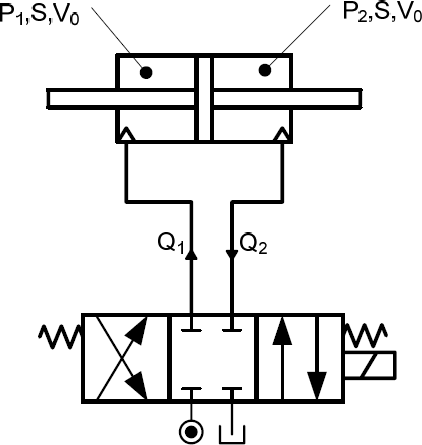
\includegraphics[width=.5\linewidth]{img_01}
\caption{RobuROC 6 \label{fig:01}}
\end{figure}

Les déplacements de la plate-forme sont coordonnés par l’intermédiaire de deux microcontrôleurs placés dans les podes avant et arrière. Ces microcontrôleurs communiquent entre eux et dialoguent avec l’extérieur suivant deux modes de conduite : 
\begin{itemize}
\item le mode joystick : l’utilisateur pilote manuellement la plate-forme par l’intermédiaire d’une télécommande;
\item le mode automatique : la plate-forme traite les informations du logiciel de supervision notamment le suivi d’un profil théorique.
\end{itemize}

Pour se repérer dans l’espace, la plate-forme est équipée de capteurs relatifs positionnés sur chacune des six roues, d’inclinomètres et d’un système de positionnement absolu par GPS. Des capteurs à ultrasons et des « bumpers » (détecteurs de collision) participent à la sécurité matérielle et à la détection des obstacles.
La motorisation principale est assurée par six moteurs électriques équipés de réducteurs épicycloïdaux permettant de transmettre l’énergie mécanique aux six roues. Le franchissement des obstacles est facilité par un système hydraulique permettant le soulèvement des podes avant et arrière. Ce système est constitué de quatre vérins disposés de part et d’autre du pode central (\autoref{fig:03}) et d’une centrale hydraulique alimentée par une pompe à engrenage (annexe 2). La plate-forme peut se déplacer, sous conditions, en mode 6 roues ou 4 roues pour certaines applications particulières (\autoref{fig:02}). L’énergie électrique nécessaire au fonctionnement est stockée dans des batteries occupant la plus grande partie du volume interne des trois podes. Une unité de gestion électrique optimise la consommation d’énergie. 

\begin{figure}
\centering
\begin{subfigure}{0.3\textwidth}
    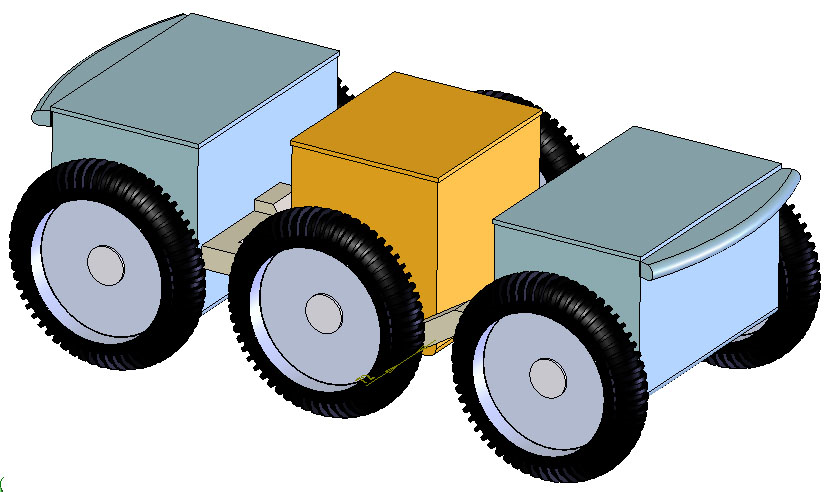
\includegraphics[width=\linewidth]{img_02_a}
    \caption{Mode 6 roues}
    \label{fig:02a}
\end{subfigure}
\begin{subfigure}{0.3\textwidth}
    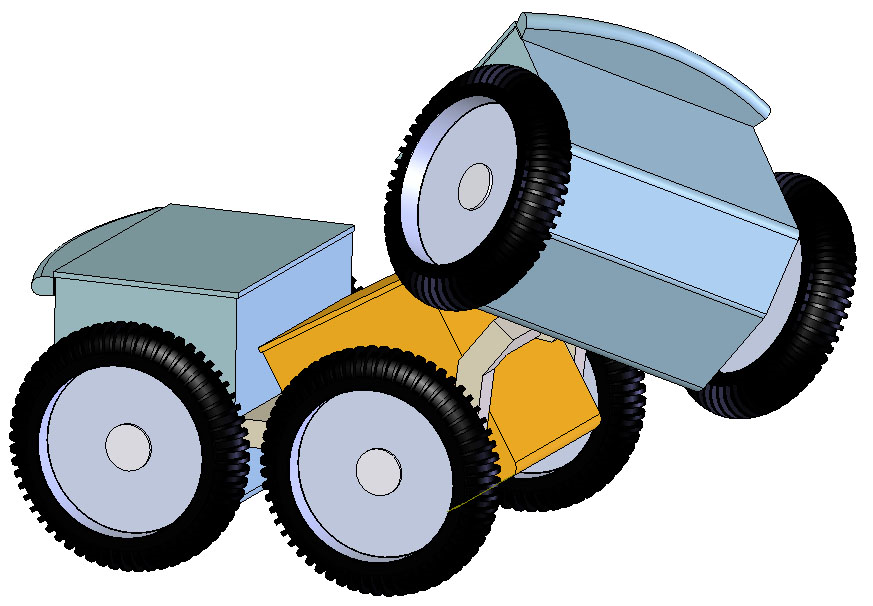
\includegraphics[width=\linewidth]{img_02_b}
    \caption{Mode 4 roues -- Déplacement}
    \label{fig:02a}
\end{subfigure}
\begin{subfigure}{0.3\textwidth}
    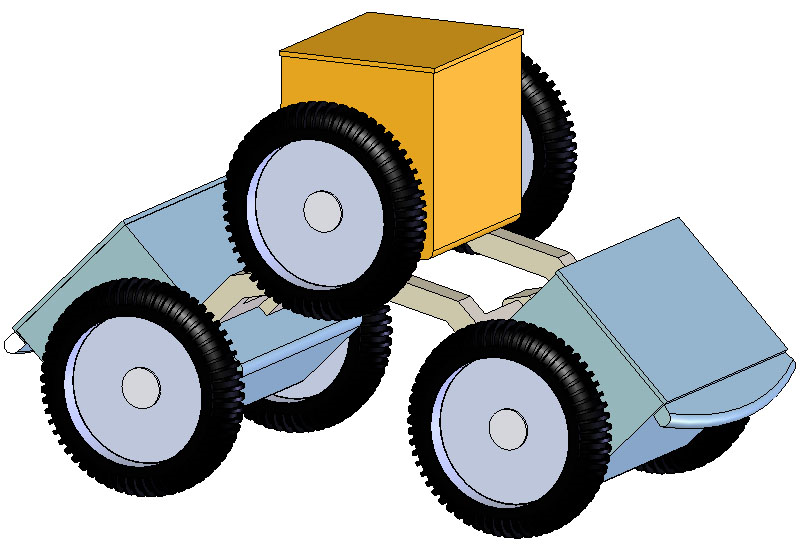
\includegraphics[width=\linewidth]{img_02_c}
    \caption{Mode 4 roues -- Observation}
    \label{fig:02a}
\end{subfigure}\caption{Mode de déplacement de la plate-forme \label{fig:02}}
\end{figure}


\begin{figure}
\centering
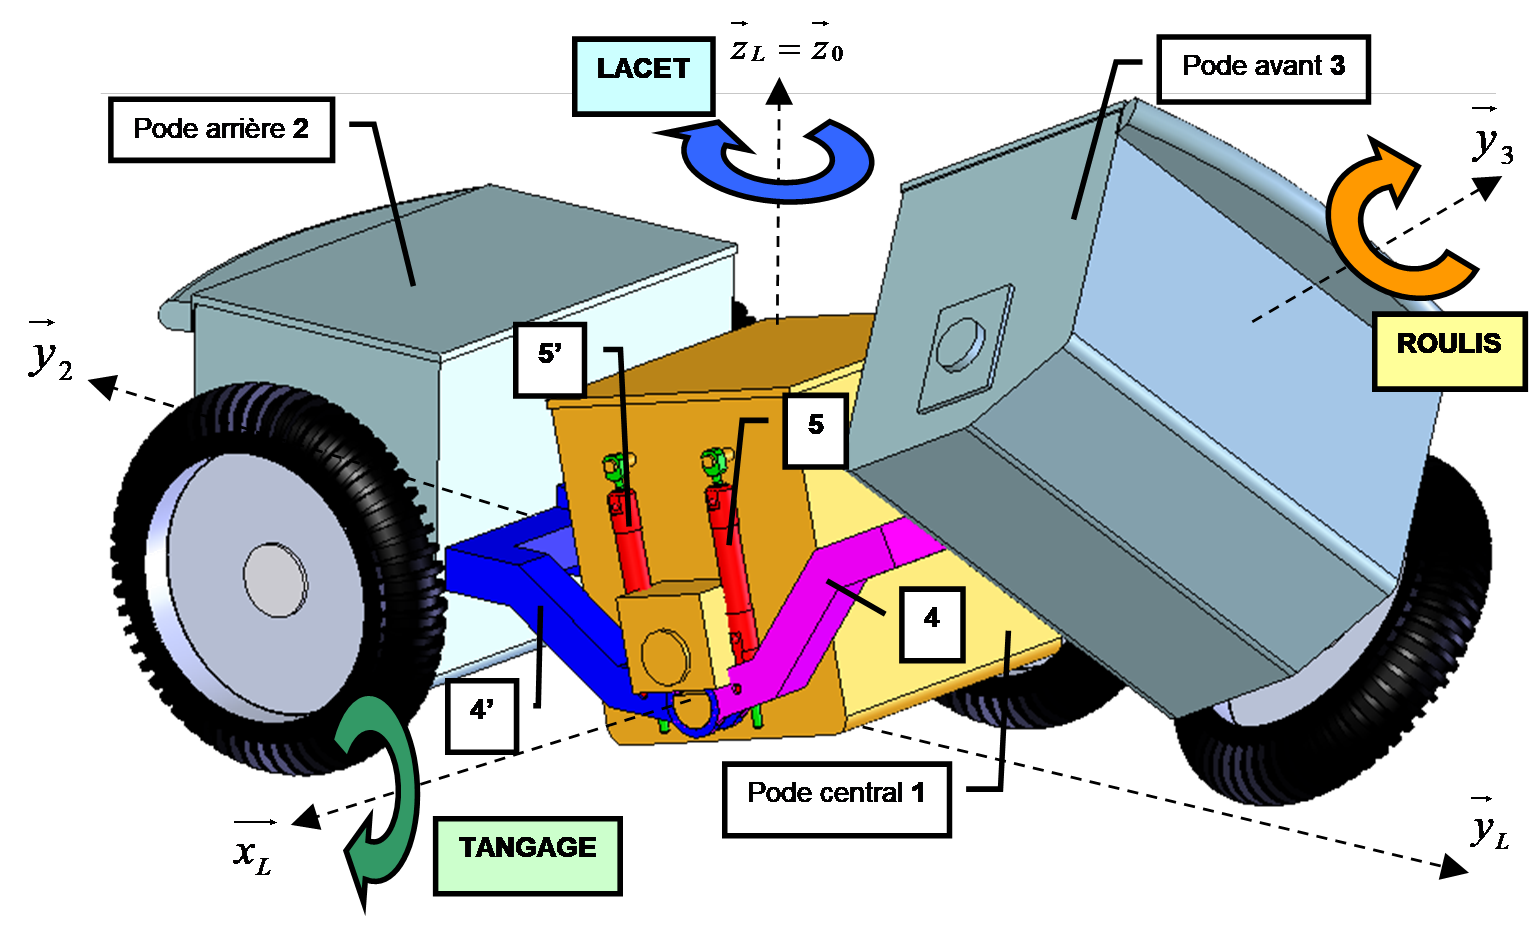
\includegraphics[width=.85\linewidth]{img_03}
\caption{Roue centrale et roue avant droite supprimées pour plus de visibilité \label{img:03}}
\end{figure}

Les trois podes sont articulés en tangage et en roulis (\autoref{fig:03}). Le mouvement de tangage est guidé par deux liaisons pivot (d’axe de direction  $\vect{x_L}$), respectivement entre le bras d’articulation avant \textbf{4} et le pode central \textbf{1} et entre le bras d’articulation arrière \textbf{4’} et le pode central \textbf{1}. Le système hydraulique de suspension permet l’amortissement (mode passif) et la motorisation de ce mouvement (mode actif). Les vérins \textbf{5} (côté droit) et \textbf{6} (côté gauche) sont en liaison avec le bras d’articulation avant \textbf{4} et le pode central \textbf{1}. Les vérins \textbf{5’} (côté droit) et \textbf{6’} (côté gauche) sont en liaison avec le bras d’articulation arrière \textbf{4’} et le pode central \textbf{1}. Le mouvement de roulis est assuré par deux liaisons pivot entre le pode avant \textbf{3} et le bras d’articulation avant \textbf{4} (liaison d’axe de direction $\vect{y_3}$) d’une part, et entre le pode arrière \textbf{2} et le bras d’articulation arrière \textbf{4’}  (liaison d’axe de direction $\vect{y_2}$) d’autre part. Ce mouvement n’est pas motorisé. 

\begin{table}
\centering
\begin{tabular}{|p{5cm}|p{5cm}|l|l|}
\hline
Fonctions & Critères & Niveaux & Flexibilité \\ 
\hline
\hline
FT3 : Assurer le déplacement	
 & Vitesse de déplacement de la plate-forme & $\SI{13,7}{km/h}$ & Valeur maximale \\ \cline{2-4}
 & Hauteur de franchissement d’un obstacle de type « trottoir » ($D_{\text{max}}$) & \SI{40}{cm} & Valeur minimale  \\ \cline{2-4}
 & Pente du relief à vide & 45\degres & Valeur maximale  \\ \cline{2-4}
 & Débattement angulaire en tangage du bras 4 par rapport au pode central 1 & de $-45\degres$ à $+30\degres$ & -----  \\ \cline{2-4}
 & Débattement angulaire en tangage du bras 4’ par rapport au pode central 1 & de $+45\degres$ à $-30\degres$ & ----- \\ \cline{2-4}
 & Débattement angulaire en roulis du pode avant 3 par rapport au bras 4 & de $-45\degres$ à $+45\degres$ & ----- \\ \cline{2-4}
 & Débattement angulaire en roulis du pode arrière 2 par rapport au bras 4’ & de $+45\degres$ à $-45\degres$ & ----- \\
 \hline
FT4 : Analyser la zone géographique à explorer
 & Charge utile répartie sur les trois podes & \SI{100}{kg} & Valeur maximale \\ \hline
 & Hauteur d’observation ($H_{\text{obs}}$) & \SI{85}{cm} & Valeur minimale \\ \hline
FT6 : Fournir l’énergie électrique & Autonomie d’utilisation $\SI{4}{h} $ & $\pm \SI{1}{h}$ & selon les conditions \\ \hline
\end{tabular}
\caption{Extrait du cahier des charges fonctionnel (d’après le diagramme FAST en annexe 1)}
\end{table}

\section{Analyse fonctionnelle}
\subparagraph{}\textit{Compléter le diagramme FAST de la plate-forme d’exploration présenté en annexe 1 en indiquant les solutions techniques associées aux fonctions techniques référencées dans le tableau du document-réponse.}
